\usetikzlibrary{arrows.meta}
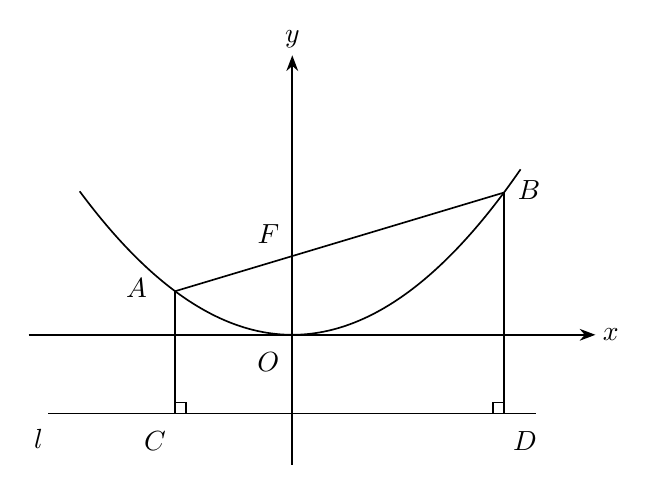
\begin{tikzpicture}[x=1cm,y=1cm,line width=.6pt,font=\normalsize,>=Stealth,
  axis/.style={->,line width=.6pt},curve/.style={line width=.6pt},segment/.style={line width=.6pt},label/.style={inner sep=1pt}]
\def\qq{4}
\coordinate (O) at (0.0,0.0);
\coordinate (F) at (0.0,1.0);
\coordinate (A) at (-1.488061,0.553582);
\coordinate (B) at (2.688061,1.806418);
\coordinate (C) at (-1.488061,-1.0);
\coordinate (D) at (2.688061,-1.0);
\coordinate (X1) at (-3.1,-1.0);
\coordinate (X2) at (3.1,-1.0);
\coordinate (AX1) at (-3.35,0.0);
\coordinate (AX2) at (3.85,0.0);
\coordinate (AY1) at (0.0,-1.65);
\coordinate (AY2) at (0.0,3.55);
\draw[axis] (AX1)--(AX2);
\draw[axis] (AY1)--(AY2);
\draw[curve] plot[domain=-2.7:2.9,samples=180,variable=\t] ({\t},{(\t*\t)/\qq});
\draw[segment] (X1)--(X2);
\draw[segment] (A)--(C);
\draw[segment] (B)--(D);
\draw[segment] (A)--(B);
\draw[segment] (C) ++(0.14,0) -- ++(0,0.14) -- ++(-0.14,0);
\draw[segment] (D) ++(-0.14,0) -- ++(0,0.14) -- ++(0.14,0);
\node[label,anchor=north east] at (-0.12,-0.18) {$O$};
\node[label,anchor=south east] at (-0.12,1.12) {$F$};
\node[label,anchor=east] at (-1.8,0.6) {$A$};
\node[label,anchor=west] at (2.82,1.84) {$B$};
\node[label,anchor=north east] at (-1.56,-1.18) {$C$};
\node[label,anchor=north west] at (2.76,-1.18) {$D$};
\node[label,anchor=north east] at (-3.12,-1.16) {$l$};
\node[label,anchor=west] at (3.9,0.0) {$x$};
\node[label,anchor=south] at (0.0,3.6) {$y$};
\end{tikzpicture}
